\documentclass[uplatex,dvipdfmx,ja=standard]{bxjsarticle}
\usepackage{amsmath,amssymb}
\usepackage{bm}
\usepackage{graphicx}
\usepackage{ascmac}
\usepackage{titlesec}
\usepackage{pdfpages}
\usepackage{listings,jvlisting}
\usepackage{url}
%
\setlength{\textwidth}{\fullwidth}
\setlength{\textheight}{40\baselineskip}
\addtolength{\textheight}{\topskip}
\setlength{\voffset}{-0.2in}
\setlength{\topmargin}{0pt}
\setlength{\headheight}{0pt}
\setlength{\headsep}{0pt}
%
\newcommand{\divergence}{\mathrm{div}\,}  %ダイバージェンス
\newcommand{\grad}{\mathrm{grad}\,}  %グラディエント
\newcommand{\rot}{\mathrm{rot}\,}  %ローテーション
%

\lstset{
  basicstyle={\ttfamily},
  identifierstyle={\small},
  commentstyle={\smallitshape},
  keywordstyle={\small\bfseries},
  ndkeywordstyle={\small},
  stringstyle={\small\ttfamily},
  frame={tb},
  breaklines=true,
  columns=[l]{fullflexible},
  numbers=left,
  xrightmargin=0zw,
  xleftmargin=3zw,
  numberstyle={\scriptsize},
  stepnumber=1,
  numbersep=1zw,
  lineskip=-0.5ex
}

\title{フーリエ解析 期末課題}
\subtitle{離散コサイン変換の応用例,jpeg変換}
\author{機械科学•航空宇宙学科 1w192224 田久健人}
\date{\today}

\begin{document}
\maketitle

\thispagestyle{empty}
\vspace{2cm}

\begin{center}
    \textbf{\Large 目       次}  
\end{center}

\renewcommand{\contentsname}{}
\tableofcontents

\newpage
\setcounter{page}{1}

\section{目的}

普段我々が身近に利用しているDCT変換の一種であるjpegについて,DTC変換の理論背景と,理論背景に基づいた簡易的な二次元配列の変換の実装の二つの観点から理解を深める.

\section{DCTの理論}
\subsection{DFT}

DCT(離散コサイン変換)を理解するにあたり,まずDFT(離散フーリエ変換)の基礎理論を整理する.

波形$f(t)$を周期$\tau$でサンプリングすると,$f(n\tau)$と表せる.

このとき,周期関数$f(t)$は,

\begin{equation}
    \label{exp:syuuki}
    f_{\tau}(t) = \sum_{n= 0}^{N-1} f(n\tau) \delta (t - n\tau)
\end{equation}

と表せる.ここで,(\ref{exp:syuuki})にFourier変換を適用すると,

\begin{equation}
    \label{exp:foo}
    \begin{split}
        F_{\tau} (f) &= \int_{-\infty}^{\infty} f_{\tau}(t)^{-j\omega t} dt \\ 
                     &= \int_{-\infty}^{\infty} \sum_{n=0}^{N-1} f(n\tau) \delta (t - n\tau)^{- j\omega t} dt \\
                     &= \sum_{n=0}^{N-1} f(n\tau) e^{-j\omega n \tau} 
    \end{split}
\end{equation}

$\omega = \frac{2 \pi k}{n \tau}$,$k = 0,1,...,N-1$より,

\begin{equation}
    \label{exp:dft}
    F_{\tau} (k) = \sum_{n=0}^{N-1} W_N ^{nk}
\end{equation}
\begin{center}
    ($W_N = e^{j \frac{1 \pi }{N}} $)
\end{center}



\subsection{DCT}

$f_{\tau}$を,中央線対象のデータに拡張する.
$f'_{\tau} = f_{\tau}(0),f_{\tau}(1),...,f_{\tau}(N-2),f_{\tau}(N-1),f_{\tau}(N-1),f_{\tau}(N-2),...,f_{\tau}(1),f_{\tau}(0)$ 
のように定義する.

$f'_{\tau}$のDFTに対し,$w(k) = e^{-j\frac{\pi }{2N}k}$をかけ,式を展開する.

\begin{equation}
    \label{exp:kakutyou}
    \begin{split}
        F'_{\tau}(k)w(k) &= \sum_{n=0}^{2N-1} f'_{\tau}(n) e^{-j\frac{\pi}{N} nk } e^{-j \frac{\pi}{2N}k} \\
                         &= \sum_{n=0}^{N-1} f'_{\tau}(n) e^{-j\frac{\pi}{2N}(2n + 1)k } + \sum_{n=N}^{2N-1} f'_{\tau}(n) e^{-j \frac{\pi}{N}(2n + 1)k}
\end{split}
\end{equation}

\newpage

$f'_{\tau}$の対称性より,

\begin{equation}
    \sum_{n=N}^{2N-1} f'_{\tau}(n) e^{-j\frac{\pi}{2N}(2n + 1)k} = \sum_{n=0}^{N -1} f'_{\tau}(n) e^{j\frac{\pi}{2N}(2n + 1)k}
\end{equation}

よって,(\ref{exp:kakutyou})は,

\begin{equation}
    \begin{split}
        F_{\tau}(k) w(k) &= \sum_{n=0}^{N-1}f'_{\tau}(n) e^{-j\frac{\pi}{2N}(2n+1)k} + \sum_{n=0}^{N-1} f'_{\tau}(n) e^{j\frac{\pi}{2N}(2n+1)k} \\
                         &= \sum_{n=0}^{N-1} f'_{\tau} (n) \left\{e^{-j \frac{\pi}{2N}(2n+1)k} + e^{j \frac{\pi}{2N}(2n+1)k} \right\} \\
                         &= 2 \sum_{n=0}^{N-1} f'_{\tau}(n) \cos{\left( \frac{\pi}{2N} (2n+1)k \right)} 
    \end{split}
\end{equation}

$N= 0,1,...,N-1$で$f'_{\tau} = f_{\tau}$より,

\begin{equation}
    \label{exp:dtc}
    F_{\tau}(k) w(k) = 2 \sum_{n=0}^{N-1} f_{\tau}(n) \cos{\left( \frac{\pi}{2N} (2n + 1)k \right)}
\end{equation}

このような,データを$1/2$で右にシフトして,前半分を離散フーリエ変換したものは,離散コサイン変換の中でも.DCT-IIと呼ばれる.DCTには他にも複数種類存在するが,その中でもDCT-IIは信号の圧縮分野で多く用いられる.

\section{画像圧縮の実装}

\subsection{二次元の対象への応用}

(\ref{exp:dtc})で示したDCTを,画像に対して利用することを考える.

\subsubsection{二次元のDFT}

まず,DFTを二次元に拡張し,行列表示することを考える.フーリエ変換の次元を増やして,

\begin{equation}
    F_{\tau}(u,v) = \int_{-\infty}^{\infty} \int_{-\infty}^{\infty} f_{\tau}(x,y) e^{-j 2\pi (ux + vy)} dxdy
\end{equation}

指数関数の性質から,
\begin{equation}
    F_{\tau}(u,v) = \int_{-\infty}^{\infty} \left[ \int_{-\infty}^{\infty} f_{\tau}(x,y) e^{-j 2\pi ux} dx \right] e^{-j 2\pi vy} dy
\end{equation}

のように分離可能である.これを離散化して,

\begin{equation}
    F_{\tau}(u,v) = \sum_{n=0}^{N-1} f(x,y) e^{-j 2\pi \frac{u}{N}x} \sum_{n=0}^{N-1} e^{-j 2\pi \frac{v}{N}y}
\end{equation}

行列表示を考える.

変換対象を$f$,DFCの行列表示を$R$,変換後を$F$とすると,$F = Rf$と表す.$R$は,


\begin{equation}
    R = \frac{1}{N}
    \label{exp:mat_dft}
        \begin{pmatrix}   
            W_N^0  & W_N^0        & W_N^0         & \ldots  &  W_N^0     \\
            W_N^0  & W_N^{-1}     & W_N^{-2}      & \ldots  & W_N^{-(N-1)}  \\
            W_N^0  & W_N^{-2}     & W_N^{-4}      & \ldots  & W_N^{-2(N-1)}  \\
            \vdots & \vdots       & \vdots        &         & \vdots \\
            W_N^0  & W_N^{-(N-1)} & W_N^{-2(N-1)} & \ldots  & W_N^{-(N-1)(N-1)}
    \end{pmatrix}
\end{equation}

このとき,$W_N = e^{-j\frac{2\pi}{N}}$とおいている.

$\mathrm{rank}R = N$より,Rは正則である.

逆変換は,Rが正則であることから,Rの逆行列を左からかけることに相当する.

\subsubsection{二次元のDCT}

同様の手順でDCTを行列で表現する.

DTCの行列表示$R$は,

\begin{equation}
    R =
    \label{exp:base}
        \begin{pmatrix}   
\ddots &           &        \\
       & \phi(k,i) &        \\
       &           & \ddots         
        \end{pmatrix}
\end{equation}

\begin{displaymath}
\phi(k,i)=
\left\{
\begin{array}{ll}
    \frac{1}{\sqrt{N}} & (k=0) \\
    \sqrt{\frac{2}{N}} \cos \frac{(2i+1)k\pi}{2N} & (k = 1,2,...,N-1)
\end{array}
\right.
\end{displaymath}

である.DCTでは複素数だった部分が実部のみで表されている.

\subsection{二次元配列に対するDCTの実装}

(\ref{exp:base})までの理論式を,pythonで愚直に実装する.

ソース全体は\url{https://github.com/tkyawa/fourier-report/tree/main/src}を別途参照する.

まず,基底関数(\ref{exp:base})を表現する.

\begin{lstlisting}[caption=dct.phi]
def phi(k, N):
    if k == 0:
        return np.ones(N)/np.sqrt(N)
    else:
        return np.sqrt(2.0/N)*np.cos((k*np.pi/(2*N))*(np.arange(N)*2+1))
\end{lstlisting}

次に,基底関数を用いて二次元の基底ベクトルを出力する関数を用意する.
\newpage

\begin{lstlisting}[caption=dct.base]
def base(N):
    phi_1 = np.array([phi(i,N) for i in range(N)])
    phi_2 = np.zeros((N, N, N, N))
    for i in range(N):
        for j in range(N):
            phi_i, phi_j = np.meshgrid(phi_1[i], phi_1[j])
            phi_2[i, j] = phi_i*phi_j
    return phi_2
\end{lstlisting}


基底関数を使って一次元の基底ベクトルphi\_1を定義した後,一次元の基底ベクトル2つを格子状に配置して,二次元の基底ベクトルとした.

次に,基底ベクトルを用いてDCTを行う関数を実装する.

\begin{lstlisting}[caption=dct.dct]
def dct(original_data, N):
    return np.sum(base(N).reshape(N*N, N*N)*original_data.reshape(N*N), axis=1).reshape(N, N)
\end{lstlisting}

基底ベクトルbase(N)に元のデータをかけあわせている.

次に,逆変換を行う関数を実装する.

\begin{lstlisting}[caption=dct.idct]
def idct(tranced_data, N):
    return np.sum((tranced_data.reshape(N, N, 1)*base(N).reshape(N,N, N*N)).reshape(N*N, N*N), axis=0).reshape(N, N)
\end{lstlisting}


必要な関数群が揃ったので,テストを行う.今回は,対象がただの二次元配列なのに加え,愚直に実装した影響でサイズ$N$が30程度しか取れないため,手動でテスト画像に変わる行列を用意する.

\begin{lstlisting}[caption=main.py]
N = 10
original_img = np.array([
	[0,0,0,0,0,0,0,0,0,0],
	[0,0,0,1,1,1,1,0,0,0],
	[0,0,1,1,0,0,1,1,0,0],
	[0,1,1,1,0,0,1,1,1,0],
	[0,1,0,0,1,1,0,0,1,0],
	[0,1,0,0,1,1,0,0,1,0],
	[0,1,1,1,0,0,1,1,1,0],
	[0,0,1,1,0,0,1,1,0,0],
	[0,0,0,1,1,1,1,0,0,0],
	[0,0,0,0,0,0,0,0,0,0]
])
base = dct.base(N)
transed_img = dct.dct(original_img,N)
resorted_img = dct.idct(transed_img, N)
\end{lstlisting}

\newpage

サイズNを10と定めた後,手動で10$\times $10のテスト行列original\_imgを用意し,先に用意した各関数に値を与えて,original\_imgに対しDCT,逆変換をする.
最後に,変換前,変換後の行列に対し,PyPlotのimshowによって画像形式で表示し,見た目を比較する.



変換前のimg,逆変換後のimgを図\ref{figure:test}に示す.

\begin{figure}[htb]
    \centering
    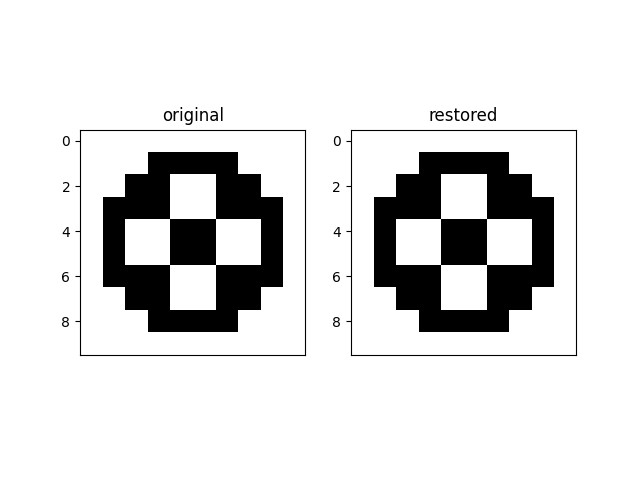
\includegraphics[scale=0.9]{../src/img/test.png}
    \caption{テスト実行結果}
    \label{figure:test}
\end{figure}

変換前に対して目視では違いがわからない程度の画像が得られているのがわかる.

\newpage

また,N=10の場合の基底ベクトルphi\_2dのimshow()による出力を図\ref{figure:base}に示す.


\begin{figure}[htb]
    \centering
    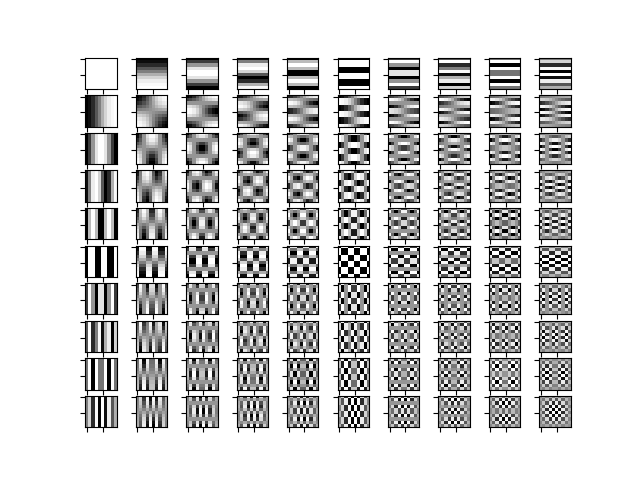
\includegraphics[scale=0.9]{../src/img/base.png}
    \caption{基底ベクトル(N=10)}
    \label{figure:base}
\end{figure}


入力画像を,これらの画像(基底ベクトル)の重ね合わせで表現している.これにより,実際のピクセルデータと比べて少ないデータ量で画像を評伝できることが期待される.

\newpage

\subsection{実際のjpeg変換}

先の実装では,が,実際の画像は座標データに加えて色を表すデータも存在するため,もう少し複雑になる.図\ref{figure:jpg}に,簡単な流れを示す.

\begin{figure}[htb]
    \centering
    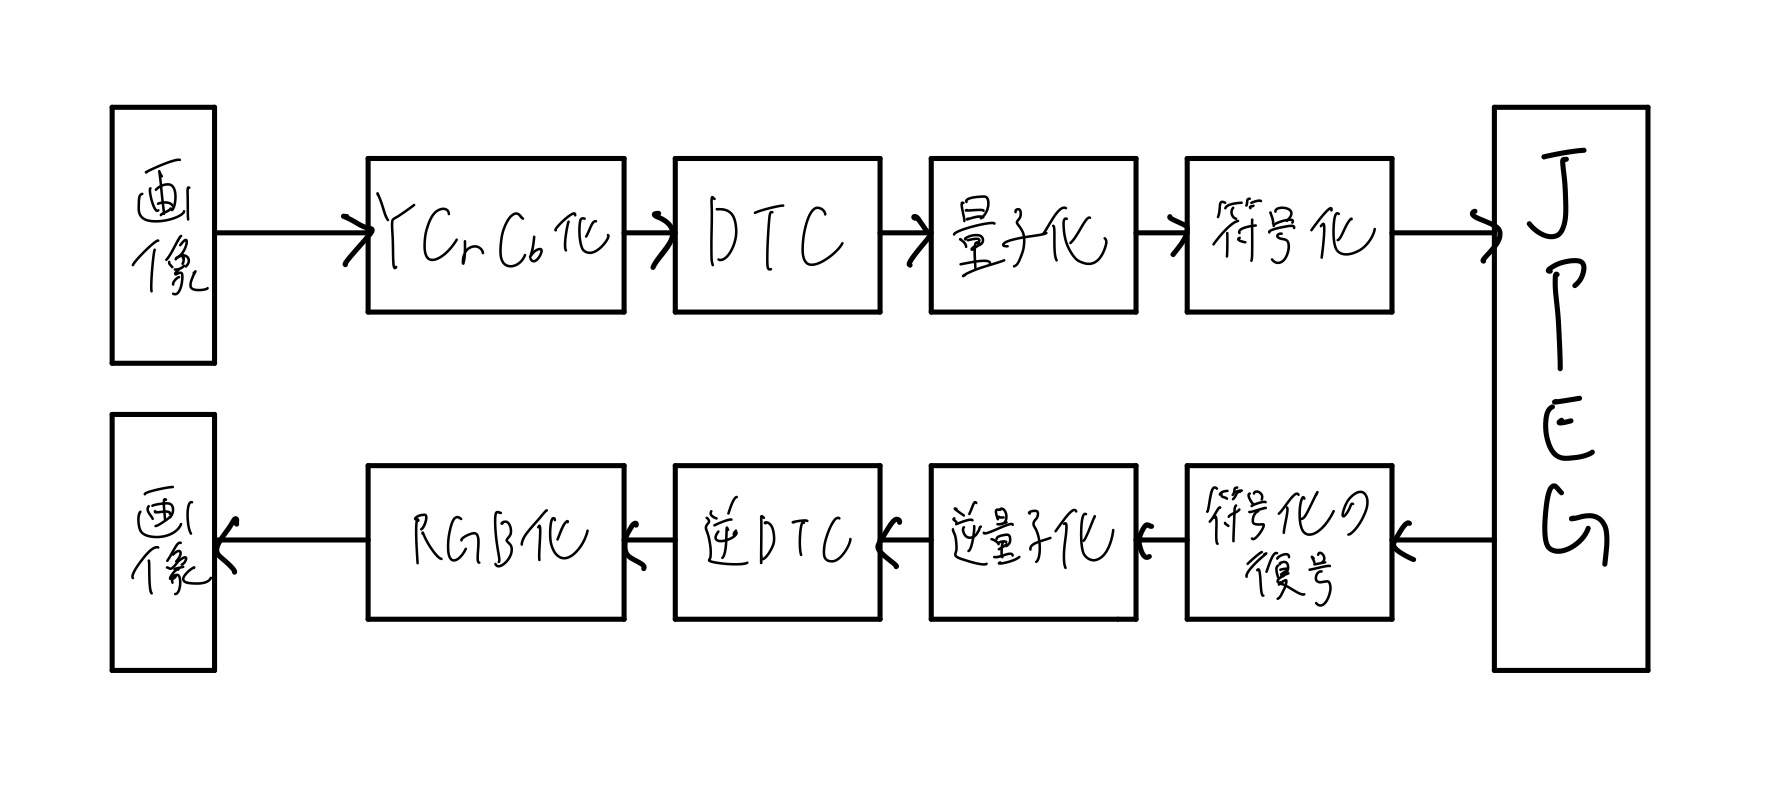
\includegraphics[scale=0.23]{img/jpeg.jpg}
    \caption{jpeg変換のフロー}
    \label{figure:jpg}
\end{figure}

\subsubsection{RGBデータの$YC_r C_b$形式への変換}

まず,元の画像を,RGB形式よりも処理が容易な$YC_rC_b$形式に変換する.このとき,
\begin{equation}
    \begin{split}
        Y &= 0.299R + 0.587G + 0.114B -128 \\
        C_b &= -0.1687R - 0.3313G + 0.5B + 128 \\
        C_r &= 0.5R - 0.4187G - 0.0813B + 128
    \end{split}
\end{equation}

の公式を用いることができる.

\subsubsection{$YC_rC_b$形式のデータのサンプリング}

データ削減のために,色素情報を1ピクセルおきに間引きする.輝度の情報のブロックに対する赤方向,青方向の情報ブロックの数の割合を$4:1:1$とする.

\subsubsection{DCT}

DCTを,8ピクセル四方単位で行う.

\subsubsection{データの量子化}

DCTによって出た細かい誤差を切り捨て,あらかじめ与えられる量子化テーブルをもとに周波数成分を64段階に分ける.jpeg画像におけるボヤけの大半は,この量子化が原因である.

\subsubsection{データの整列}

変換後の$8\times 8$のデータを一列に並べ直す.行列の0番成分を基点とし,ジグザグスキャンと呼ばれる規則により一列にする.


\subsubsection{データの符号化}

エントロピー符号化をすることにより,データを圧縮する.

\subsubsection{データの復号}

符号化に用いた符号表を用いて復号,量子化に用いた量子テーブルをもとに逆量子化を行う.その後,逆DCTを行い,もとのデータを取り出す.


\section{文献}
1) 大石進一,"フーリエ解析",(2007) 岩波書店

2) \url{https://www.onosokki.co.jp/HP-WK/eMM_back/emm138.pdf}

最終アクセス:2021年12月29日

3) \url{https://www.marguerite.jp/Nihongo/Labo/Image/JPEG.html}

最終アクセス:2021年12月30日

4) \url{http://racco.mikeneko.jp/Kougi/2016a/IPPR/2016a_ippr09_slide_ho.pdf}

最終アクセス:2021年12月30日

5) \url{https://tony-mooori.blogspot.com/2016/02/dctpythonpython.html}

最終アクセス:2021年12月30日

6) 酒井幸市,"画像処理とパターン認識入門",(2006),共立出版 

%\begin{table}[ht]
%    \caption{}
%    \label{table:}
%    \centering
%    \begin{tabular}{c | c | c}
%     \hline \hline
%     \hline
%    \end{tabular}
%\end{table}



%\begin{figure}[htb]
%    \centering
%    \includegraphics[scale=0.23]{1.png}
%    \caption{}
%    \label{figure:}
%\end{figure}

%\includepdf{hoge-hyousi.pdf}
%


%
%
\end{document}

%%% End:
